\documentclass[../admech.tex]{subfiles}
\begin{document}
\section{Conservation Laws}% and Noether's Theorem}
\subsection{Conservation of Generalized Energy and Generalized Momentum}
All conservation laws can be determined again in Lagrangian mechanics using the symmetries of the Lagrangian. This comes from a really important theorem, called \emph{Noether's theorem} which briefly states that for every continuously differentiable symmetry of the Lagrangian there exists a conservation law.\\
\begin{dfn}[Integral of Motion]
	An \emph{integral of motion} or \emph{first integral} are all the quantities which depend only on the generalized coordinates and their derivatives $(q^\mu,\dot{q}^\mu)$.\\
	Since they're time independent, we have that the integral $k_{(i)}$ is a conserved quantity, since
	\begin{equation*}
		\dv{k_{(i)}}{t}=0
	\end{equation*}
\end{dfn}
We begin by stating the first two main simmetries that pop out from the properties of space and time itself, like isotropy and homogeneity.
\begin{thm}[Conservation of Energy]
	Given an isolated system with Lagrangian $\lag(q^\mu,\dot{q}^\mu)$ not subject to dissipative forces, due to the homogeneity of time, the generalized energy $E(q^\mu,\dot{q}^\mu,t)$ defined as
	\begin{equation}
		E(q^\mu,\dot{q}^\mu)=\dot{q}^\mu\pdv{\lag}{\dot{q}^\mu}-\lag(q^\mu,\dot{q}^\mu)
		\label{eq:genenergy}
	\end{equation}
	Is an integral of motion
\end{thm}
\begin{proof}
	We begin by finding the total time derivative of the Lagrangian. The differential of the Lagrangian is
	\begin{equation*}
		\dd{\lag}=\pdv{\lag}{q^\mu}\dd{q^\mu}+\pdv{\lag}{\dot{q}^\mu}\dd{\dot{q}^\mu}
	\end{equation*}
	Therefore
	\begin{equation*}
		\dot{\lag}=\pdv{\lag}{q^\mu}\dot{q}^\mu+\pdv{\lag}{\dot{q}^\mu}\ddot{q}^\mu
	\end{equation*}
	Substituting the first term on the RHS with the Euler Lagrange equation $\dv{t}\dot{\del}_\mu\lag=\del_\mu\lag$, where with $\dot{\del}_\mu$ we indicate the derivative with respect to the velocities, we have
	\begin{equation*}
		\dot{\lag}=\dv{t}\pdv{\lag}{\dot{q}^\mu}\dot{q}^\mu+\pdv{\lag}{\dot{q}^\mu}\ddot{q}=\dv{t}\left( \dot{q}^\mu\pdv{\lag}{\dot{q}^\mu} \right)
	\end{equation*}
	Moving the terms around, we have
	\begin{equation*}
		\dv{t}\left( \dot{q}^\mu\pdv{\lag}{\dot{q}^\mu}-\lag \right)=\dv{E}{t}=0
	\end{equation*}
	Which states that $E(q^\mu,\dot{q}^\mu)$ is an integral of motion since it's conserved.
\end{proof}
Note the previous definition of the energy. Since $\dot{q}^\mu\dot{\del_\mu}\lag=\dot{q}^\mu\dot{\del_\mu}T=2T$, we have
\begin{equation*}
	E(q^\mu,\dot{q}^\mu)=2T(q^\mu,\dot{q}^\mu)-T(q^\mu,\dot{q}^\mu)+\pot(q^\mu)
\end{equation*}
Therefore, we end up to the usual definition of energy
\begin{equation}
	E(q^\mu,\dot{q}^\mu)=T(q^\mu,\dot{q}^\mu)+\pot(q^\mu)
	\label{eq:genenergyis}
\end{equation}
Another integral of motion can be determined from the properties of space
\begin{thm}[Conservation of Momentum]
	Due to the homogeneity of space, the quantity $p_\mu$ called \emph{generalized momentum}
	\begin{equation}
		p_\mu=\dot{\del}_\mu\lag
		\label{eq:genmom}
	\end{equation}
	Is an integral of motion
\end{thm}
\begin{proof}
	The homogeneity of space implies that for a parallel translation of all the points of a system the Lagrangian is invariant. Therefore for an infinitesimal translation $q^\mu\to q^\mu+\delta q^\mu$ where $\delta q^\mu\le\epsilon$ we have
	\begin{equation*}
		\delta\lag=\pdv{\lag}{q^\mu}\delta q^\mu=0
	\end{equation*}
	Therefore, using Euler-Lagrange equations
	\begin{equation*}
		\dv{t}\pdv{\lag}{\dot{q}^\mu}=\dv{p_\mu}{t}=0
	\end{equation*}
	Which proves the theorem. This, also implies that, again using Euler-Lagrange
	\begin{equation*}
		\dv{p_\mu}{t}=\pdv{\lag}{q^\mu}=Q_\mu=0
	\end{equation*}
	Which implies that the system is in equilibrium
\end{proof}
\begin{exe}[Application of Conservation Laws]
	A quick way to show the importance of conservation laws is a simple exercise, that can be found at pg. 46 \cite{landau1}.\\
	Suppose that a particle with mass $m$ and initial velocity $v_1$ is moving in a potential field $\pot_1$, which after passing a wall changes to $\pot_2$.\\
	Find the change in direction of the velocity.
	\begin{figure}[H]
		\centering
		\begin{tikzpicture}
			\draw[->] (0,-1) -- (0,3) node[right] {\small$\pot$};
			\draw[->] (-3,0) -- (3,0) node[below] {\small$r$};
			\draw (1,0.1) -- (1,-0.1) node[below] {\small$r_w$};
			\draw[dashed] (1,0.1) -- (1,3);
			\draw[domain=-3:1] plot (\x,1);
			\draw[domain=1:3] plot (\x,2.5);
			\node at (-1.5,1.2) {\small$\pot_1$};
			\node at (2,2.7) {\small$\pot_2$};
		\end{tikzpicture}
		\caption{The piecewise potential $\pot(r)$}
		\label{fig:piecpot}
	\end{figure}
	Changing immediately to the orthogonal system of coordinates formed by the normal and tangent  to the wall $q^\mu=(n,t)$ we have that
	\begin{equation*}
		\del_t\pot=-\del_t\lag=0
	\end{equation*}
	Therefore, using Euler-Lagrange equations we immediately know that in these coordinates
	\begin{equation*}
		\dot{p}_t=0
	\end{equation*}
	This implies therefore that the generalized momentum projected onto the tangent to the plane will be conserved going through the wall, and therefore
	\begin{equation*}
		v_1^t=v_2^t
	\end{equation*}
	Now we might have two cases
	\begin{enumerate}
	\item The particle is already moving normally to the wall, hence $v_1^t=v_2^t=0$
	\item The particle is moving with an angle $\theta$ to the wall, hence $v_1\sin\theta=v_2\sin\eta$
	\end{enumerate}
	The second case can be illustrated in this drawing\\
	\begin{minipage}[c]{0.5\textwidth}
		\begin{figure}[H]
			\centering
			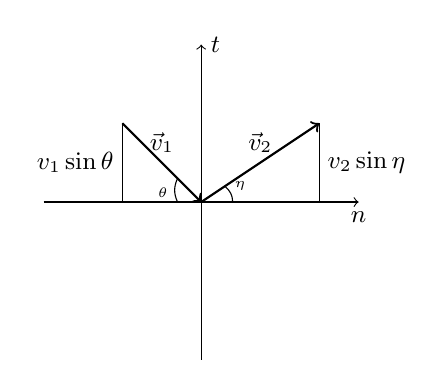
\begin{tikzpicture}
				\draw[->] (0,-2) -- (0,2) node[right] {\small$t$};
				\draw[->] (-2,0) -- (2,0) node[below] {\small$n$};
				\draw[->,thick] (-1,1) -- (0,0);
				\draw[->, thick] (0,0) -- (1.5,1);
				\draw (-0.3,0) to [bend left=25] (-0.3,0.3) node[below left] {\tiny$\theta$};
				\draw (0.4,0) to [bend right=25] (0.3,0.2) node[right] {\tiny$\eta$};
				\draw (-1,1) -- (-1,0);
				\draw (1.5,1) -- (1.5,0);
				\node at (-1.6,0.5) {\small$v_1\sin\theta$};
				\node at (2.1,0.5) {\small$v_2\sin\eta$};
				\node[above] at (-0.5,0.5) {\small$\vec{v}_1$};
				\node[above] at (0.75,0.5) {\small$\vec{v}_2$};
			\end{tikzpicture}
			\caption{Incidence angle of the particle}
			\label{fig:incang}
		\end{figure}
	\end{minipage}\begin{minipage}[c]{0.5\textwidth}
		Using the previous equation we have that
		\begin{equation*}
			\frac{\sin\theta}{\sin\eta}=\frac{v_2}{v_1}
		\end{equation*}
		For determining the velocities we use the conservation of energy, which gives
		\begin{equation*}
			T_1+\pot_1=T_2+\pot_2
		\end{equation*}
	\end{minipage}\\
	Therefore solving for $T_2/T_1$ we get
	\begin{equation*}
		\frac{T_2}{T_1}=1+\frac{1}{T_1}(\pot_1-\pot_2)
	\end{equation*}
	Substituting $T=mv^2/2$ we have finally
	\begin{equation*}
		\frac{v^2_2}{v^2_1}=1+\frac{2}{mv^2_1}(\pot_1-\pot_2)
	\end{equation*}
	I.e., taking the square root
	\begin{equation*}
		\frac{\sin\theta}{\sin\eta}=\pm\sqrt{1+\frac{2}{mv^2_1}(\pot_1-\pot_2)}
	\end{equation*}
	This is finally the change in direction of the particle in passing through the wall
\end{exe}
\subsection{Change of Inertial Reference Frames}
The behavior of Lagrangians and therefore action, in change of reference frames isn't hard to grasp.\\
Suppose there is a system of particles with masses $m_i$ and velocities $v_{(i)}^\mu$ in some reference frame $K$. Changing to a second reference frame $\tilde{K}$ moving with velocity $V^\mu$ we have that the velocities transform with the following law
\begin{equation}
	v^\mu_{(i)}=\tilde{v}_{(i)}^\mu+V^\mu
	\label{eq:lagvintrlaw}
\end{equation}
\begin{figure}[H]
	\centering
	\begin{tikzpicture}
		%K
		\draw[->] (-5,-1) -- (-5,0) node[left] {\tiny$z$};
		\draw[->] (-5,-1) -- (-4,-1) node[below] {\tiny$x$};
		\draw[->] (-5,-1) -- (-5.85,-1.53) node[right] {\tiny$y$};
		\node[below ] at (-5,-1) {\small$K$};
		%K'
		\draw[->,dashed] (-5,-1) -- (0,0) node[below] {\small$\tilde{K}$};
		\draw[->] (0,0) -- (1.3,1.3);
		\node[above] at (0.5,0.5) {\small$V^\mu$};
		\draw[->] (0,0) -- (0,1) node[left] {\tiny$\tilde{z}$};
		\draw[->] (0,0) -- (1,0) node[below] {\tiny$\tilde{x}$};
		\draw[->] (0,0) -- (-0.85,-0.52) node[right] {\tiny$\tilde{y}$};
	\end{tikzpicture}
	\caption{The reference frames $K$ and $\tilde{K}$}
	\label{fig:reframestrans}
\end{figure}
If we write the total momentum of the system as $P^\mu=\sum m_iv^\mu_{(i)}$, we have that the momentum changes with the following law
\begin{equation}
	P^\mu=\sum_im_i\tilde{v}^\mu_{(i)}+V^\mu\sum_im_i=\tilde{P}^\mu_{(i)}+MV^\mu
	\label{eq:lagpintrlaw}
\end{equation}
This tells us immediately that we can find a system such that $\tilde{P}^\mu=0$, therefore, in this system
\begin{equation}
	P^\mu=MV^\mu
	\label{eq:lagcmtr}
\end{equation}
The velocity of the system we're searching depends therefore on the masses, and we get
\begin{equation}
	V^\mu=\frac{P^\mu}{M}
	\label{eq:vcmlag}
\end{equation}
This can be seen as the total derivative of the radius vector of the center of mass.\\
Writing energy as $T+\pot$ we have that it changes between inertial reference frames as follows
\begin{equation}
	E=\frac{1}{2}\sum_im_i(\tilde{v}^\mu_{(i)}+V^\mu)^2+\pot=\frac{1}{2}\sum_im_i\tilde{v}^2+V^\mu\tilde{P}_\mu+\frac{1}{2}MV^2+\pot
	\label{eq:lagencm}
\end{equation}
Writing $E_{int}=\tilde{T}+\pot$ as the \emph{internal energy} of the system, we have that, in the system of the center of mass
\begin{equation}
	E=E_{int}+\frac{1}{2}MV^2
	\label{eq:cmen}
\end{equation}
\begin{exe}[Transformation of Action Between Inertial Frames]
	A nice way for seeing these transformations in action is seeing how the action transforms between inertial reference frames, as in the problem at pg. 48 \cite{landau1}.\\
	Since we know already that
	\begin{equation}
		T=\tilde{T}+\frac{1}{2}MV^2+V^\mu\tilde{P}_\mu
		\label{eq:kinenintr}
	\end{equation}
	We have that the Lagrangian $\lag=T-\pot$ changes as follows
	\begin{equation}
		\lag=\tilde{T}+\frac{1}{2}MV^2+V^\mu\tilde{P}_\mu-\pot=\tilde{\lag}+\frac{1}{2}MV^2+V^\mu\tilde{P}_\mu
		\label{eq:lagintr}
	\end{equation}
	Integrating the Lagrangian with respect to time, we have
	\begin{equation*}
		\act=\int_{}^{}\lag\dd{t}=\int_{}^{}\tilde{\lag}\dd{t}+V^\mu\int\tilde{P}_\mu\dd{t}+\frac{1}{2}MV^2\int_{}^{}\dd{t}
	\end{equation*}
	Integrating directly, and putting $\tilde{P}^\mu=M\dv{t}\tilde{X}^\mu$, we have
	\begin{equation}
		\act=\tilde{\act}+MV^\mu\tilde{X}_\mu+\frac{1}{2}MV^2t
		\label{eq:actintr}
	\end{equation}
\end{exe}
\subsection{Conservation of Angular Momentum}
\begin{thm}[Conservation of Angular Momentum]
	Due to the isotropy of space, the properties of a system are invariant to rotations, and the angular momentum $L_\mu$ defined as
	\begin{equation*}
		L_\mu=\epsilon_{\mu\nu\sigma}x^\nu p^\sigma
	\end{equation*}
\end{thm}
\begin{proof}
	Take a system with radius vector $x^\mu$ and apply some rotation vector $\delta\varphi^\mu$, the system will rotate of an angle $\theta$ and have a linear displacement $\delta x^\mu$ as in the following figure
	\begin{figure}[H]
		\centering
		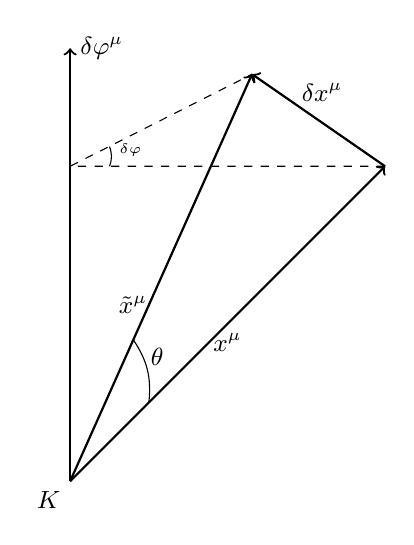
\begin{tikzpicture}
			\draw[->,thick] (0,0) -- (0,5.5) node[right] {\small$\delta\varphi^\mu$};
			\draw[->,thick] (0,0) -- (4,4);
			\node[below] at (2,2) {\small$x^\mu$};
			\draw[->,thick] (0,0) -- (2.31,5.17);
			\node[above] at (0.8,2) {\small$\tilde{x}^\mu$};
			\draw[->,thick] (4,4) -- (2.31,5.17);
			\node[above] at (3.2,4.7) {\small$\delta x^\mu$};
			\draw (0.8,1.8) to [bend left=20] (1,1);
			\node[above right] at (0.9,1.35) {\small$\theta$};
			\draw[dashed] (4,4) -- (0,4) -- (2.31,5.17);
			\draw (0.5,4.25) to [bend left=20] (0.5,4) node [above right] {\tiny$\delta\varphi$};
			\node[below left] at (0,0) {\small$K$};
		\end{tikzpicture}
		\caption{Uniform rotation of the system by an angle $\delta\varphi$}
		\label{fig:rotvec}
	\end{figure}
	By the right hand rule we have
	\begin{equation}
		\norm{\delta x}=\norm{x}\norm{\delta\varphi}\sin\theta
		\label{eq:normdeltaxrot}
	\end{equation}
	This implies, again by the right hand rule that
	\begin{equation}
		\delta x^\mu=g^{\mu\nu}\epsilon_{\nu\gamma\sigma}\delta\varphi^\gamma x^\sigma
		\label{eq:deltaxmuvec}
	\end{equation}
	Using the fact that $\delta\varphi^\mu$ is constant, we have that the variation of the velocity of the system is
	\begin{equation}
		\delta v^\mu=g^{\mu\nu}\epsilon_{\nu\gamma\sigma}\delta\varphi^\gamma v^\sigma
		\label{eq:velvar}
	\end{equation}
	Shoving it all in the variation of the Lagrangian $\delta\lag$ and imposing its invariance, we have
	\begin{equation}
		\begin{aligned}
			\delta\lag&=\pdv{\lag}{x^\mu}\delta x^\mu+\pdv{\lag}{v^\mu}\delta v^\mu\\
			\delta\lag&=\pdv{\lag}{x^\mu}g^{\mu\nu}\epsilon_{\nu\gamma\sigma}\delta\varphi^\gamma x^\sigma+\pdv{\lag}{v^\mu}g^{\mu\nu}\epsilon_{\nu\gamma\sigma}\delta\varphi^\gamma v^\sigma=0
		\end{aligned}
		\label{eq:lagvarang}
	\end{equation}
	Substituting $\del_\mu\lag=\dot{p}_\mu$ and $\dot{\del}_\mu\lag=p_\mu$ we have, after a cyclic exchange of indexes
	\begin{equation}
		\delta\varphi^\mu\left( \epsilon_{\mu\nu\gamma}x^\nu\dot{p}^\gamma+\epsilon_{\mu\nu\gamma}v^\nu p^\gamma \right)=0
		\label{eq:var}
	\end{equation}
	Noting that inside there is actually a total derivative of a product, we can write
	\begin{equation}
		\delta\varphi^\mu\dv{t}\left( \epsilon_{\mu\nu\gamma}x^\nu p^\gamma \right)=\dv{L_\mu}{t}\delta\varphi^\mu=0
	\end{equation}
	Which is the searched integral of motion.
\end{proof}
In a change of inertial reference frames $K\to\tilde{K}$, where $\tilde{K}$ is moving with velocity $V^\mu$, the angular momentum transforms as
\begin{equation}
	L_\mu=\tilde{L}_\mu+\epsilon_{\mu\nu\sigma}X^\nu P^\sigma
	\label{eq:angmomchange}
\end{equation}
Since
\begin{equation*}
	L_\mu=\sum_im_i\epsilon_{\mu\nu\sigma}x^\nu_{(i)}\tilde{v}_{(i)}^\sigma+\sum_{i}m_i\epsilon_{\mu\nu\sigma}x^\nu_{(i)}V^\sigma
\end{equation*}
\subsection{Noether's Theorem}
In general all conservation laws can be condensed in one single theorem that works on the symmetries of the Lagrangian, this really important theorem is known as \emph{Noether's theorem} and ties the invariance of the Lagrangian to the integrals of motion.\\
\begin{thm}[Noether's Theorem]
	Given any transformation of coordinates $q^\mu\to q^\mu+\delta q^\mu,\ \delta q^\mu\propto\epsilon$ which is related to a symmetry of the Lagrangian implies that the equation of motion are invariant and there exists a conserved quantity associated to the symmetry
\end{thm}
\begin{proof}
	We begin the proof by applying the transformation to the Lagrangian. We obtain, using the fact that the transformation is infinitesimal
	\begin{equation*}
		\delta\lag(q^\mu+\delta q^\mu,\dot{q}^\mu+\delta\dot{q}^\mu,t)\simeq\delta\lag+c_1\delta q^\mu+c_2\delta\dot{q}^\mu
	\end{equation*}
	If this transformation is a symmetry transformation of the Lagrangian we have that
	\begin{equation*}
		\lag(q^\mu+\delta q^\mu,\dot{q}^\mu+\delta\dot{q}^\mu,t)=\lag(q^\mu,\dot{q}^\mu+\delta\dot{q}^\mu,t)\implies c_1=0
	\end{equation*}
	Therefore, integrating over time we get the associated variated action
	\begin{equation*}
		\delta\act=\int_{t_1}^{t_2}\delta\lag\dd{t}+\int_{t_1}^{t_2}c_2\delta\dot{q}^\mu\dd{t}
	\end{equation*}
	Using the usual boundary conditions of the least action theorem, and noting that the first term in the RHS must be zero in order to satisfy Euler-Lagrange equations, we have
	\begin{equation*}
		\delta\act=\left[c_2\delta q^\mu\right]_{t_1}^{t_2}-\int_{t_1}^{t_2}\dot{c}_2\delta q^\mu\dd{t}=-\int_{t_1}^{t_2}\dot{c}_2\delta q^\mu\dd{t}=0
	\end{equation*}
	Therefore, for the first theorem of variational calculus we have
	\begin{equation*}
		\dot{c}_2=0
	\end{equation*}
	Which implies that $c_2$ is an integral of motion, derived from a symmetry transformation.\\
	Note that if the transformation isn't a symmetry transformation we get
	\begin{equation*}
		\dot{c}_2=c_1
	\end{equation*}
	Therefore $c_2$ isn't generally an integral of motion
\end{proof}
\section{Mechanical Similarity}
Due to the invariance of the Euler-Lagrange equations to the multiplication of constants, we might imagine to use this property to our advantage with some kind of coordinate transformation.\\
Suppose that the potential function $\pot$ is $k$-homogeneous, which means
\begin{equation*}
	\pot(\alpha q^\mu)=\alpha^k\pot(q^\mu)
\end{equation*}
These kinds of potentials are actually common in physics as we will see later, but in order to showcase this method of mechanical similarity we apply the following transformation
\begin{equation}
	\left\{ \begin{aligned}
			q^\mu&\to\alpha\tilde{q}^\mu\\
			t&\to\beta\tilde{t}
	\end{aligned}\right.
	\label{eq:mechsimtrans}
\end{equation}
This gives us that $\dot{q}^\mu\propto\frac{\alpha}{\beta}\dot{\tilde{q}}^\mu$, and due to the shape of the kinetic energy we get
\begin{equation*}
	T\propto\frac{\alpha^2}{\beta^2}\tilde{T}
\end{equation*}
Now, we have that the parameter $\alpha$ is fixed from the potential energy itself, while the second parameter $\beta$, for now, is free. In order to fix that parameter we must impose the invariance of the equation of motion, i.e. impose that
\begin{equation*}
	\lag=\alpha^k\tilde{\lag}
\end{equation*}
This is pretty easy to impose, we simply need that both the new modified kinetic energy and potential energy are multiplied by the same parameter $\alpha^k$, and therefore
\begin{equation}
	\frac{\alpha^2}{\beta^2}=\alpha^k\implies\beta=\alpha^{1-\frac{k}{2}}
	\label{eq:betafixmechsim}
\end{equation}
This leaves the equations of motion unchanged, but also simplified. Other things that this brings is the possibility to write relations between quantities. We have, if we write the linear path length as $l$, that
\begin{equation}
	\frac{\tilde{t}}{t}=\left( \frac{\tilde{l}}{l} \right)^{1-\frac{k}{2}}
	\label{eq:mechsimrel}
\end{equation}
Therefore, we also have for velocity, energy and length
\begin{equation}
	\frac{\tilde{v}}{v}=\left( \frac{\tilde{l}}{l} \right)^{\frac{k}{2}}\qquad\frac{\tilde{E}}{E}=\left( \frac{\tilde{l}}{l} \right)^{k}\qquad\frac{\tilde{L}}{L}=\left( \frac{\tilde{l}}{l} \right)^{1+\frac{k}{2}}
	\label{eq:mechsimrel2}
\end{equation}
Applying this to a Coulombian potential $\pot(r)=k/r$, we have, if the field is attractive, i.e. $k=-1$
\begin{equation}
	\frac{\tilde{t}}{t}=\left( \frac{\tilde{l}}{l} \right)^{\frac{3}{2}}
	\label{eq:kepler3mechsim}
\end{equation}
Which is simply the square root of Kepler's third law.
\subsection{Virial Theorem}
Using the techniques of mechanical similarity, there's a theorem which pops out quite easily, the virial theorem.\\
\begin{thm}[Virial Theorem]
	Suppose that the motion of a system happens in a limited space, therefore $\dot{x}^\mu\dot{\del}_\mu T=2T$. If $\tilde{\pot}=k\pot$ then
	\begin{subequations}
		\begin{equation}
			\expval{T}=\frac{k}{2}\pot
			\label{eq:virialthm}
		\end{equation}
		And
		\begin{equation}
			\left\{ \begin{aligned}
					\expval{T}&=\frac{k}{k+2}\expval{E}\\
					\expval{\pot}&=\frac{2}{k+2}\expval{E}
			\end{aligned}\right.
			\label{eq:virialthm2}
		\end{equation}
	\end{subequations}
\end{thm}
\begin{proof}
	Since the motion is in a limited space, we have that $\dot{x}^\mu\dot{\del}_\mu T=\dot{x}^\mu p_\mu=2T$, and applying the time average, we have
	\begin{equation*}
		\expval{2T}=\lim_{\tau\to\infty}\frac{2}{\tau}\left(\int_{0}^{\tau}\dv{t}p_\mu x^\mu\dd{t}-\int_{0}^{\tau}x^\mu\dot{p}_\mu\dd{t}\right)
	\end{equation*}
	From Euler-Lagrange tho, we also have that $x^\mu\dot{p}_\mu=-x^\mu\del_\mu\pot$, and therefore, since the first integral is null
	\begin{equation*}
		\expval{2T}=\expval{x^\mu\del_\mu\pot}
	\end{equation*}
	If the potential is $k$-homogeneous, we have
	\begin{equation*}
		\expval{T}=\frac{k}{2}\expval{\pot}
	\end{equation*}
	Since the total energy in this case is constant and conserved, we must have
	\begin{equation*}
		\expval{T}+\expval{\pot}=E
	\end{equation*}
	Substituting the previous result, we have
	\begin{equation*}
		\frac{k}{2}\expval{\pot}+\expval{\pot}=E
	\end{equation*}
	Solving for $\expval{\pot}$ we have the first result
	\begin{equation*}
		\expval{\pot}=\frac{2}{k+2}E
	\end{equation*}
	Inserting again the first result
	\begin{equation*}
		\expval{T}=\frac{k}{k+2}E
	\end{equation*}
\end{proof}
\section{Integration of the Equations of Motion}
\subsection{Unidimensional Motion}
The integration of the equations of motion isn't always direct, but it's definitely easier when the considered system only has one degree of freedom $q(t)$. The most general Lagrangian of such system has the following shape
\begin{equation*}
	\lag(q,\dot{q},t)=\frac{1}{2}a(q)\dot{q}^2-\pot(q)
\end{equation*}
If $q(t)=x(t)$ we have that $a(q)=m$, and therefore
\begin{equation*}
	\lag(x,\dot{x},t)=\frac{1}{2}m\dot{x}^2-\pot(x)
\end{equation*}
Without even writing the equations of motion we begin to write a differential equation starting from the first possible integral of motion, $E$.
\begin{equation*}
	E=\frac{1}{2}m\dot{x}^2-\pot(x)
\end{equation*}
Solving for $\dot{x}$ the result is a first-order separable differential equation
\begin{equation}
	\dv{x}{t}=\sqrt{\frac{2}{m}\left( E-\pot(x) \right)}
	\label{eq:fsde1m}
\end{equation}
From this we have two immediate solutions
\begin{equation}
	\begin{aligned}
		x(t)&=\sqrt{\frac{2}{m}}\int_{t_0}^{t}\sqrt{E-\pot(x)}\dd{t}\\
		t(x)&=\sqrt{\frac{m}{2}}\int_{x_0}^{x}\frac{1}{\sqrt{E-\pot(x)}}\dd{x}
	\end{aligned}
	\label{eq:solde1m}
\end{equation}
Since $x(t)$ must be real, the motion is therefore possible only in the regions where $E\ge\pot(x)$. The points where $E=\pot(x)$ are called \emph{stopping points}, i.e. where $\dot{x}=0$.\\
If we have that $x(t)$ is limited between two stopping points $x_{s_0}$ and $x_{s_1}$, the motion is said to be \emph{limited} between these points, or \emph{infinite} otherwise.\\
The nature of limited motion is inherently oscillatory, contained inside a potential hole or potential well.\\
The period of the oscillation of the system from the first stopping point till the second is quite easy to calculate. Taking the second expression in equation \eqref{eq:solde1m} and fixing the integration extremes between the two stopping points and multiplying by $2$, we have the period of the system in function to the total energy of the system
\begin{equation}
	T(E)=\sqrt{2m}\int_{x_{s_1}}^{x_{s_2}}\frac{1}{\sqrt{E-\pot(x)}}\dd{x}
	\label{eq:periodenergy}
\end{equation}
\subsection{Motion in a Central Field}
\begin{dfn}[Reduced Mass]
	Suppose that two particles are moving in a field where $\pot=\pot(\norm{r_1^\mu-r_2^\mu}_\mu)$, i.e. the field depends only on the distance between the two particles. It's possible then to reduce the problem with the following coordinate transformation
	\begin{equation}
		\left\{ \begin{aligned}
			r^\mu&=r^\mu_1-r_2^\mu\\
			\tilde{P}^\mu&=m_1r^\mu_1+m_2r^\mu_2=0
		\end{aligned}\right.
		\label{eq:rmtrans}
	\end{equation}
	This reduces the Lagrangian to the motion of only the center of mass of the two particles, where
	\begin{equation*}
		\lag(r^\mu,\dot{r}^\mu)=\frac{1}{2}\mu \dot{r}^\mu\dot{r}_\mu-\pot(r)
	\end{equation*}
	The parameter $\mu$ is known as \emph{reduced mass} of the system, where
	\begin{equation*}
		\mu=\frac{1}{\frac{1}{m_1}+\frac{1}{m_2}}=\frac{m_1m_2}{m_1+m_2}
	\end{equation*}
	The inverse transformation is immediately retrieved from the system \eqref{eq:rmtrans}, where
	\begin{equation*}
		\left\{ \begin{aligned}
				r^\mu_1&=\frac{m_2}{m_1+m_2}r^\mu\\
				r^\mu_2&=-\frac{m_1}{m_1+m_2}r^\mu
		\end{aligned}\right.
	\end{equation*}
\end{dfn}
The notion of reduced mass is extremely useful in treating central force fields, i.e. forces that have the same direction of the radius of a circle. Considering a conservative force and polar coordinates we have that such force can be expressed as follows
\begin{equation*}
	F^\mu=-g^{\mu\nu}\del_\nu\pot=-\dv{\pot}{r}\frac{\hat{r}^\mu}{r}
\end{equation*}
In this case we also have that $L_\mu\perp r^\mu$, and the Lagrangian of such system has the following shape
\begin{equation*}
	\lag(r,\dot{r},\varphi,\dot{\varphi})=\frac{1}{2}m(\dot{r}^2+r^2\dot{\varphi}^2)-\pot(r)
\end{equation*}
The absence of a direct dependence of the Lagrangian from the coordinate $\varphi$ gives an immediate conservation law, where
\begin{equation*}
	\del_\varphi\lag=\dot{p}_\mu=0
\end{equation*}
This coordinate is called \emph{cyclic}, and corresponds to another conservation law
\begin{equation*}
	\pdv{\lag}{\dot{\varphi}}=mr^2\dot{\varphi}=L_z
\end{equation*}
Which, written explicitly using Euler-Lagrange equations, gives
\begin{equation*}
	\dot{p}_\varphi=\del_\varphi\lag=\dot{L}_z=0
\end{equation*}
Identifying both $L_z$ and $p_\varphi$ as integrals of motion.\\
The geometrical interpretation of this is quite easy. Define the area spanned by a particle moving in this field, going from $r^\mu$ to $r^\mu+\dd{r^\mu}$, calling this area $\dd{A}$ we have
\begin{equation}
	\dd{A}=\frac{1}{2}mr^2\dd{\varphi}
	\label{eq:infareacpot}
\end{equation}
Linking that to our previous integral of motion, we have
\begin{equation}
	L_\mu=2m\dot{A}
	\label{eq:angmomareacpot}
\end{equation}
This implies that also $2m\dot{A}$ must be constant, and it's simply \emph{Kepler's second law of orbital motion}. Looking back at the relation between $\dot{\varphi}$ and $L_z$ we can say
\begin{equation}
	\dot{\varphi}^2=\frac{L_z^2}{m^2r^4}
	\label{eq:philzcpot}
\end{equation}
Which lets us rewrite the Lagrangian in a different fashion
\begin{equation}
	\lag=\frac{1}{2}m\dot{r}^2+\frac{L^2}{2mr^2}-\pot(r)
	\label{eq:effpotlag}
\end{equation}
The integration of these equations of motion is pretty easy, and remembering that the ``new'' part that we added \emph{isn't} a piece of the potential, gives the following energy expression.
\begin{equation}
	E=\frac{1}{2}m\dot{r}^2+\frac{L_z^2}{2mr^2}+\pot(r)
	\label{eq:energycpot}
\end{equation}
Solving for $\dot{r}$ we have a slightly modified version of what we saw for general one dimensional motion
\begin{equation}
	\begin{aligned}
		r(t)&=\int_{t_1}^{t_2}\sqrt{\frac{2}{m}(E-\pot(r))-\frac{L_z^2}{m^2r^2}}\dd{t}\\
		t(r)&=\int_{r_1}^{r_2}\frac{1}{\sqrt{\frac{2}{m}(E-\pot(r))-\frac{L_z^2}{m^2r^2}}}\dd{r}
	\end{aligned}
	\label{eq:rttrcpot}
\end{equation}
Using (again) the cyclic variable, we have that $\dd{\varphi}=\frac{L_z}{mr^2}\dd{t}$ we can rewrite the second integral in a more convenient way, as
\begin{equation}
	\varphi(r)=\int_{r_1}^{r_2}\frac{L_z}{mr^2}\frac{1}{\sqrt{\frac{2}{m}(E-\pot(r))-\frac{L_z^2}{m^2r^2}}}\dd{r}=\int_{r_1}^{r_2}\frac{L_z}{r^2}\frac{\dd{r}}{\sqrt{2m(E-\pot(r))-\frac{L^2_z}{r^2}}}
	\label{eq:orbiteq}
\end{equation}
This is extremely convenient since it gives the general solution to our problem, and also the equation of the trajectory of the system in this central field.\\
Another way to treat this is by defining a ``new'' \emph{effective potential} $\pot_{eff}$ where
\begin{equation}
	\pot_{eff}(r)=\pot(r)+\frac{L_z^2}{2mr^2}
	\label{eq:effpot}
\end{equation}
The new piece we added to this potential is known as \emph{centrifugal energy}. Note that the stopping points of this effective potential \emph{do not} coincide with the points where the system completely stops, but instead coincides with the points where only $\dot{r}$ changes sign, effectively giving the farthest and closest points of the trajectory with respect to the center of the field.\\
Note that we have an orbit around the origin of the field if and only if both the closest and farthest point coexist. This doesn't assure us that this orbit is closed tho, for this to be true we need that in going from $r_{min}$ to $r_{max}$ and back the system is again at its starting point, which is true \emph{iff}
\begin{equation}
	\Delta\varphi=2\int_{r_{min}}^{r_{max}}\frac{L_z}{r^2}\left( 2m(E-\pot(r))-\frac{L_z^2}{r^2} \right)^{-\frac{1}{2}}\dd{r}\mod{2\pi}=0
	\label{eq:closedorbit}
\end{equation}
This integral basically tells us that for having a closed orbit, the variation of the position in this trajectory after a whole revolution (i.e. going from $r_{min}$ to $r_{max}$ and back) must be 0 or an integer multiple of $2\pi$ (if we consider more than one revolution), therefore indicating that for a \emph{whole orbit}
\begin{equation}
	\Delta\varphi\propto2\pi\implies\Delta\varphi=\frac{m}{n}2\pi,\quad m,n\in\Z
	\label{eq:closedorbitprop}
\end{equation}
\subsubsection{Center Falling}
One question might arise immediately: is it possible for a system which is interacting with a central potential to fall \emph{directly} towards the center? The answer is \emph{not always}. In fact the centrifugal energy component makes it possible if and only if
\begin{equation}
	\frac{1}{2}m\dot{r}^2=E-\pot(r)>\frac{L_z^2}{mr^2}
	\label{eq:centerfallchar}
\end{equation}
Which also implies that
\begin{equation*}
	r^2\pot(r)+\frac{L_z^2}{2m}<Er^2
\end{equation*}
Or, written more conveniently, we have that a system can fall to the center, i.e. $r\to0$ is possible, if and only if
\begin{equation}
	r^2\pot(r)<-\frac{L_z^2}{2m}
	\label{eq:centerfallpot}
\end{equation}
I.e. for a Coulombian potential $\pot(r)=-\alpha/r^2$, we must have $\alpha>L_z^2/2mr^2$, or the potential is not Coulombian, where $\pot(r)\propto r^{-n}$ with $n>2$
\subsection{Kepler's Problem and Orbital Mechanics}
The best physical example of a problem where central potentials come into action is orbital mechanics in attractive fields where $\pot(r)\propto r^{-1}$, the gravitational potential is exactly one of these. We have, in this case
\begin{equation}
	\begin{aligned}
		\pot(r)&=-\frac{\alpha}{r}\\
		\pot_{eff}(r)&=\pot(r)+\frac{L^2}{2mr^2}
	\end{aligned}
	\label{eq:keplerpot}
\end{equation}
This field is notorious for diverging at $r=0$ and fading to zero as $r\to\infty$, and the minimum is
\begin{equation*}
	\min\left\{ \pot_{eff} \right\}=\pot_{eff}\left( \frac{L^2}{\alpha m} \right)=-\frac{\alpha^2 m}{2L^2}
\end{equation*}
Due to the shape of this potential, the motion considered will be finite iff $E<0$ and the trajectory equation is directly integrable
\begin{equation}
	\varphi(r)=\int_{}^{}\frac{L}{r}\left( 2mE-2m\pot(r)-\frac{L^2}{r^2} \right)^{-\frac{1}{2}}\dd{r}=\acos\left( \frac{\frac{L}{r}-\frac{m\alpha}{L}}{\sqrt{2mE+\frac{m^2\alpha^2}{L^2}}} \right)+\varphi_0
	\label{eq:orbiteqkepler}
\end{equation}
Writing $p=\frac{L^2}{m\alpha}$ and $e=\sqrt{1+\frac{2EL^2}{m\alpha^2}}$ this becomes the equation of a conic, with $p$ and $e$ as the \emph{parameter} and the \emph{eccentricity} of the orbit, giving us, finally
\begin{equation}
	\frac{p}{r}=1+e\cos(\varphi)
	\label{eq:ellipseeqorb}
\end{equation}
Note that with $E<0$ and $e<1$ this is an ellipse
\begin{figure}[H]
	\centering
	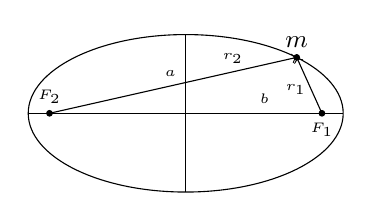
\begin{tikzpicture}
		%ellipse+focus+axes
		\draw (0,0) ellipse (2cm and 1cm);

		\draw[fill=black] (1.73,0) circle (1pt);
		\node[below] at (1.73,0) {\tiny$F_1$};
		\draw[fill=black] (-1.73,0) circle (1pt);
		\node[above] at (-1.73,0) {\tiny$F_2$};
		\draw (-2,0) -- (2,0);
		\node[above] at (1,0) {\tiny$b$};
		\draw (0,-1) -- (0,1);
		\node[left] at (0,0.5) {\tiny$a$};
		%point
		\draw[fill=black] (1.41,0.71) circle (1pt);
		\node[above] at (1.41,0.71) {\small$m$};
		%arrows
		\draw[->] (1.73,0) -- (1.41,0.71);
		\node at (1.4,0.3) {\tiny$r_1$};
		\draw[->] (-1.73,0) -- (1.41,0.71);
		\node at (0.6,0.7) {\tiny$r_2$};
	\end{tikzpicture}
	\caption{Orbit of a mass $m$ in a Keplerian potential with $E<0$ and $e<1$.}
	\label{fig:ellipseorbit}
\end{figure}
The parameters of this ellipse can be directly tied to the actual parameters of motion, using the previous definition and a bit of geometry. We have
\begin{equation}
	\begin{aligned}
		a&=\frac{p}{1-e^2}=\frac{\alpha}{2\abs{E}}\\
		b&=\frac{p}{\sqrt{1-e^2}}=\frac{L}{2m\abs{E}}
	\end{aligned}
	\label{eq:parametersellipseorbit}
\end{equation}
The minimum of the energy is reached at the same time that the effective potential has its minimum (at $r=-\alpha^2m/2L^2$). The minimum of the energy corresponds to this value iff $e=0$ and the trajectory becomes that of a circle. The farthest and closest points from the center of the field (at one of the focuses of the ellipse) are
\begin{equation}
	r_{min}=\frac{p}{1+e}=a(1-e)\qquad r_{max}=\frac{p}{1-e}=a(1+e)
	\label{eq:minmaxorbit}
\end{equation}
Which, as said before, are the roots of the equation $\pot_{eff}=E$, i.e. the ``effective'' stopping points.\\
Since as we have seen before $2m\dot{A}=L$, we have that in a complete revolution $2mA=TL$ with $A$ as the area of the ellipse. Rearranging everything into a system, we have
\begin{equation}
	\left\{ \begin{aligned}
		2m\pi ab&=TL\\
		a&=\frac{\alpha}{2\abs{E}}\\
		b&=\frac{L}{\sqrt{2m\abs{E}}}
	\end{aligned}\right.
	\label{eq:systemkepler3}
\end{equation}
Substituting, we have that
\begin{equation*}
	T=\frac{2m\pi\alpha}{2\abs{E}\sqrt{2m\abs{E}}}
\end{equation*}
Rearranging everything and making $a$ pop back again, we have
\begin{equation}
	T=2\pi a^{\frac{3}{2}}\sqrt{\frac{m}{\alpha}}
	\label{eq:kepler31/2}
\end{equation}
Squaring everything, we get back \emph{Kepler's third law of orbital motion}
\begin{equation}
	T^2=\frac{4m\pi a^3}{\alpha}\implies T^2\propto a^3
	\label{eq:kepler3complete}
\end{equation}
This can be rearranged in a different way, we begin without trying to get a relation between the period $T$ and the parameters of the ellipse ($a,b,e,p$) and we take the previous result and substitute what we found for $a$, giving us the period of the orbit with respect to the total energy of the system, as follows
\begin{equation}
	T(\abs{E})=\alpha\pi\sqrt{\frac{m}{2\abs{E}^3}}
	\label{eq:periodenergykepler}
\end{equation}
Which is just a rephrasing of Kepler's third law.\\
Going back to the conic equation for the motion in a Keplerian field, we have that for $E>0$ the motion is infinite (hyperbolic) with $e>1$. The parameters of this orbit are
\begin{equation}
	r_{min}=\frac{p}{e+1}=\frac{\alpha}{2\abs{E}}(e+1)
	\label{eq:minradhyp}
\end{equation}
Where $\alpha/2\abs{E}=a$ is the axis of the hyperbola. A particular case of this hyperbolic motion is if $E=0$ and therefore $e=1$, we have
\begin{equation}
	r_{min}=\frac{p}{2}=\frac{L^2}{2m\alpha}
	\label{eq:parthypminrad}
\end{equation}
Hyperbolic paths can be illustrated as follows
\begin{figure}[H]
	\centering
	\begin{tikzpicture}[domain=-1.5:1.5]
		\draw[->] (-1,0) -- (2,0) node[below] {$x$};
		\draw[->] (0,-2) -- (0,2) node[right] {$y$};
		\draw plot (-1.25*\x*\x+1,\x);
		\draw (1,0.1) -- (1,-0.1);
		\node[below right] at (0.9,0) {\tiny$r_{min}$};
		\draw (-0.1,0.89) -- (0.1,0.89);
		\node[right] at (0,1) {\tiny$p$};
	\end{tikzpicture}
	\caption{Hyperbolic orbit with orbital parameters, note that $r_{min}=a(e+1)$}
	\label{fig:hyperbolicorbitkepler}
\end{figure}
\end{document}
